\documentclass{article}
\usepackage{amsmath, amssymb, amsthm}
\usepackage{geometry}
\usepackage{enumitem}
\usepackage{xcolor}
\usepackage{listings}
\usepackage{bm}
\usepackage{graphicx}

\usepackage[ruled,vlined]{algorithm2e}

\geometry{a4paper, margin=1in}

\lstset{
    language=Python,
    basicstyle=\ttfamily\footnotesize,
    keywordstyle=\color{blue},
    stringstyle=\color{green},
    commentstyle=\color{gray},
    numbers=left,
    numberstyle=\tiny\color{gray},
    stepnumber=1,
    numbersep=5pt,
    showspaces=false,
    showstringspaces=false,
    breaklines=true,
    frame=single,
    captionpos=b
}

\newcommand{\py}[1]{\texttt{\lstinline!#1!}}

\title{Additional material Week 4}
\date{\vspace{-5ex}}

\begin{document}
\maketitle

\section{Question 1}
\subsection{Statement}
Apply repeatedly the 3 by 3 blurring kernel to the image of the full car plate, until the digits are no longer recognizable.

\subsection{Theory}
In order to blur the image, we replace each pixel with its average with its 8 neighbors. Averaging pixel values has the effect of smoothing the image: a light smoothing effect can be used to remove noise from an image, while a more aggressive smoothing can erase details altogether.

We formalized this procedure as a \emph{discrete convolution}, denoted with the symbol $*$, between the input image $A$ and a second matrix $K$, called \emph{kernel}: given an input image $A \in \mathbb{R}^{M \times N}$,  a kernel $K \in \mathbb{R}^{(2r +1)\times (2r+1)}$, the discrete convolution of $A$ and $K$ is an image $R \in \mathbb{R}^{(M - 2r)\times (N-2r)}$ defined as:
\begin{equation*}
    R_{i, j} = (A * K)_{i,j} = \sum_{m=0}^{2r}\sum_{n=0}^{2r} A_{i+m,j+n}K_{m,n}
\end{equation*}
The gray-level value of each pixel of the output image $R$ is the weighted sum of pixels in the $(2r+1)\times(2r+1)$ neighborhood around the corresponding pixel in the input image, with the weights equal to the elements of the kernel.

\subsection{Python solution}
To achieve this, we need to call \py{im_filtering} in a loop. At each iteration, we filter the result of the previous one after having reapplied the padding.
\lstinputlisting[language=Python, firstline=32, lastline=38]{W4Q1_multiple_blurs.py}
Listing \ref{q1pycode} shows the final Python code for the solution.
\lstinputlisting[language=Python, caption={Python code solution for the Question.}, label=q1pycode]{W4Q1_multiple_blurs.py}

\subsection{Matlab solution}
To achieve this, we need to call \py{im_filtering} in a loop. At each iteration, we filter the result of the previous one after having reapplied the padding.
\lstinputlisting[language=Matlab, firstline=11, lastline=18]{W4Q1_multiple_blurs.m}
Listing \ref{q1matcode} shows the final Matlab code for the solution.
\lstinputlisting[language=Matlab, caption={Matlab code solution for the Question.}, label=q1matcode]{W4Q1_multiple_blurs.m}

\subsection{Comments}
\begin{figure}[h]
\centering
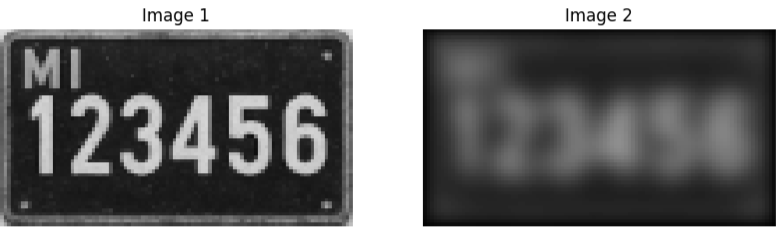
\includegraphics[width=0.85\linewidth]{W4Q1_multiple_blurs_plot.png}
\caption{Original image on the left and filtered image after applying the blur 20 times ont he right.}
\end{figure}
After 20 blurring iterations, the image has been completely blurred and the numbers are no longer recognizable.
Notice that a black outline has appeared around the image, even though the original one does not have many black pixels in that region: this is due to the black padding that has been added at each iteration. The zero padding pixels are averaged with the image ones, effectively darkening the result.
More sophisticated padding techniques can be used to avoid this effect, such as creating a padding that repeats the values of the pixels on the image border.

\section{Question 2}
\subsection{Statement}
Try blurring the image of the full car plate by applying a 5 by 5 version of the kernel seen during the lecture:
\begin{equation*}
    K = \frac{1}{25} \begin{bmatrix}
    1 & 1 & 1 & 1 & 1 \\
    1 & 1 & 1 & 1 & 1 \\
    1 & 1 & 1 & 1 & 1 \\
    1 & 1 & 1 & 1 & 1 \\
    1 & 1 & 1 & 1 & 1
    \end{bmatrix}
\end{equation*}

\subsection{Theory}
The concept is very similar to what we have done during the lecture: to blur the image we average the value of neighboring pixels, but instead of considering a 3 by 3 square we consider all pixels in a 5 by 5 square centered on the current pixel. This means that we are taking the average of 25 pixels instead of 9, and so the blurring effect will be more pronounced.
Given that a 5 by 5 kernel extends in each direction by 2 pixels from the central one, it can be applied only on those pixels that are at least 2 rows and 2 columns distant from the outside border of the image. Consequently, the resulting image will be smaller: if the original image is $M \times N$ pixels, the result will be $(M-4) \times (N-4)$. We can remedy this by padding the input image like we did in the lecture, except now the padding will be 2 pixels wide.

\subsection{Python solution}
First of all, we need to define the new blurring kernel. We can do it by creating a 5 by 5 matrix of ones and dividing it by 25: \py{K = np.ones((5, 5)) / 25}.
Next, we need to modify the \py{local_convolution} function so that it correctly loops over the bigger kernel, by using \py{range(5)} instead of \py{range(3)}. When accessing the image \py{A}, we also need to change the shift from -1 to -2 for the same reason.
\lstinputlisting[language=Python, firstline=5, lastline=10]{W4Q2_5by5_box_blur.py}
We also need to slightly modify the \py{im_filtering} function: the result is now a $(M-4) \times (N-4)$ image and the nested for loops must exclude 2 rows and 2 columns on each side of the image. The shift for saving the result in \py{R} must also be changed to -2.
\lstinputlisting[language=Python, firstline=12, lastline=20]{W4Q2_5by5_box_blur.py}
Finally, we add a bigger padding, creating a $(M+4) \times (N+4)$ image, to counteract this loss.
\lstinputlisting[language=Python, firstline=29, lastline=30]{W4Q2_5by5_box_blur.py}
Listing \ref{q2pycode} shows the final Python code for the solution.
\lstinputlisting[language=Python, caption={Python code solution for the Question.}, label=q2pycode]{W4Q2_5by5_box_blur.py}

\subsection{Matlab solution}
First of all, we need to define the new blurring kernel. We can do it by creating a 5 by 5 matrix of ones and dividing it by 25: \py{K = ones(5, 5) / 25}.
Next, we need to modify the \py{local_convolution} function so that it correctly loops over the bigger kernel, by letting \py{m} and \py{n} be equal to the range \py{1:5} instead of \py{1:3}. When accessing the image \py{A}, we also need to change the shift from -2 to -3 for the same reason.
\lstinputlisting[language=Matlab, firstline=1, lastline=8]{W4Q2_5by5_box_blur.m}
We also need to slightly modify the \py{im_filtering} function: the result is now a $(M-4) \times (N-4)$ image and the nested for loops must exclude 2 rows and 2 columns on each side of the image. The shift for saving the result in \py{R} must also be changed to -2.
\lstinputlisting[language=Matlab, firstline=10, lastline=20]{W4Q2_5by5_box_blur.m}
Finally, we add a bigger padding, creating a $(M+4) \times (N+4)$ image, to counteract this loss.
\lstinputlisting[language=Matlab, firstline=29, lastline=30]{W4Q2_5by5_box_blur.m}
Listing \ref{q2matcode} shows the final Matlab code for the solution.
\lstinputlisting[language=Matlab, caption={Matlab code solution for the Question.}, label=q2matcode]{W4Q2_5by5_box_blur.m}

\subsection{Comments}
\begin{figure}[h]
\centering
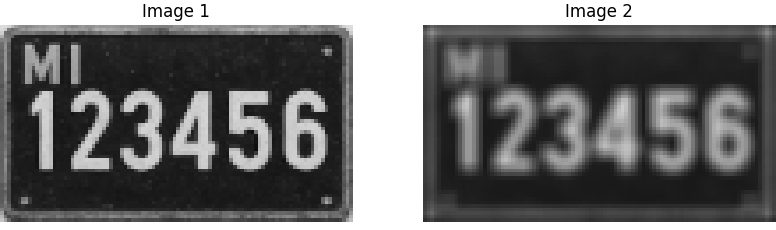
\includegraphics[width=0.85\linewidth]{W4Q2_5by5_box_blur_plot.png}
\caption{Original image on the left and filtered image on the right.}
\end{figure}
As we can see, the blur produced by the bigger 5 by 5 kernel is more noticeable because we are averaging together more pixels than before. However, it is overall still quite soft and not sufficient to hide the details in the image; a possible solution is to apply the filter multiple times like we did in the previous exercise.

\section{Question 3}
\subsection{Statement}
Try applying the following two kernels to the car plate image. Can you guess what is their intended effect?
\begin{equation*}
    K = \begin{bmatrix}
    -1 & 2 & -1 \\
    -1 & 2 & -1 \\
    -1 & 2 & -1
    \end{bmatrix} \quad
    K = \begin{bmatrix}
     0 & -1 &  0 \\
    -1 &  5 & -1 \\
     0 & -1 &  0
    \end{bmatrix}
\end{equation*}

\subsection{Theory}
The first kernel is an \emph{edge detection} filter. Intuitively, an edge is the "border" of an object, but how can we automatically find edges in an image? An edge can be described as an area characterized by a rapid change in color/intensity: inside the same object, pixel values will tend to be similar, forming uniform-looking region; on the other hand, if by moving in a particular direction we encounter a steep increase or decrease in image values, then we are likely on the border between two objects.
The rate of change of intensity can be quantified by computing the derivatives of the image using finite differences. Recall that the central finite difference formulas for estimating the first and second order derivatives of a real function are:
\begin{equation*}
    f'(x) \approx \frac{f(x+h)-f(x-h)}{2h} \ , \ f''(x) \approx \frac{f(x+h) - 2f(x) + f(x-h)}{h^2}
\end{equation*}
Notice that the weights of one row of the kernel \py{[-1, 2, -1]} are identical to the weights of the formula for $f''(x)$ (except with opposite sign)! This means that the convolution with this kernel is equivalent to computing the second partial derivative of the image in the horizontal direction. To better understand this, set the upper and lower rows of the kernel to zero:
\begin{equation*}
    \left( A *  \begin{bmatrix}
    0 & 0 & 0 \\
    -1 & 2 & -1 \\
    0 & 0 & 0 \end{bmatrix}\right)_{i, j} =
   -1 \times A_{i - 1, j} + 2 \times A_{i, j} -1 \times A_{i + 1, j}
\end{equation*}
The $h$ in the finite difference formula does not appear because it corresponds to the width of a pixel and is implicitly set to 1. Computing the horizontal derivative enables the detection of vertical edges, because an edge line is orthogonal to the direction with steepest intensity change, so the first kernel is actually a \emph{vertical edge detection} kernel, to be more precise.

The second kernel is known as a \emph{sharpening} kernel, because it enhances edges, making them "sharper".
The sharpening kernel can be decomposed as this sum:
\begin{equation*}
    \begin{bmatrix}
     0 & -1 &  0 \\
    -1 &  5 & -1 \\
     0 & -1 &  0
    \end{bmatrix} =
    \begin{bmatrix}
    0 & 0 & 0 \\
    0 & 1 & 0 \\
    0 & 0 & 0
    \end{bmatrix} +
    \begin{bmatrix}
     0 & -1 &  0 \\
    -1 &  4 & -1 \\
     0 & -1 &  0
    \end{bmatrix} = K_1 + K_2
\end{equation*}
The first kernel $k_1$ is the identity kernel, that is $A*K_1 = A$. The second $k_2$ is once again an edge detection kernel, but instead of computing the derivative of the image only in the horizontal direction, it computes the \emph{laplacian}, which is the sum of both second partial derivatives (horizontal and vertical):
\begin{equation*}
    \begin{array}{ll}
        \Delta f(x, y) = \frac{\partial^2 f}{\partial x^2} + \frac{\partial^2 f}{\partial y^2} &\approx \frac{1}{h^2}(f(x+h, y) - 2f(x, y) + (x-h, y)) + \frac{1}{h^2}(f(x, y+h) - 2f(x, y) + f(x, y-h)) = \\
        &= \frac{1}{h^2}\left(f(x+h, y) + f(x, y+h) + f(x-h, y) + f(x, y-h) -4f(x, y)\right)
    \end{array}
\end{equation*}
$K_2$ highlights all edges, not only the vertical ones. Convolving the image with $K_1 +K_2$ is the equivalent to adding the detected edges back to the original image, which in practice means that the edges get amplified, making the image sharper.

\subsection{Python solution}
Since these two kernels are 3 by 3, we can reuse the code from the lecture, changing only the definition of the convolution kernel.
In Python, we can initialize a two-dimensional array by using \py{np.array} and passing the elements as a nested list, that is a list of lists where each inner list corresponds to one row of the matrix.
\lstinputlisting[language=Python, firstline=26, lastline=35]{W4Q3_extra_kernels.py}
Then, we can just call \py{im_filtering} once for each of the kernels. Listing \ref{q3pycode} shows the final Python code for the solution.
\lstinputlisting[language=Python, caption={Python code solution for the Question.}, label=q3pycode]{W4Q3_extra_kernels.py}

\subsection{Matlab solution}
Since these two kernels are 3 by 3, we can reuse the code from the lecture, changing only the definition of the convolution kernel.
In Matlab, we can initialize a matrix by listing its elements within square brackets \py{[]} separated by whitespace, with newlines denoting the beginning of a new row. Alternatively, it is possible to use a more explicit syntax and separate elements with colons and rows with semicolons.
\lstinputlisting[language=Matlab, firstline=5, lastline=14]{W4Q3_extra_kernels.m}
Then, we can just call \py{im_filtering} once for each of the kernels. Listing \ref{q3matcode} shows the final Matlab code for the solution.
\lstinputlisting[language=Matlab, caption={Matlab code solution for the Question.}, label=q3matcode]{W4Q3_extra_kernels.m}

\subsection{Comments}
\begin{figure}[h]
\centering
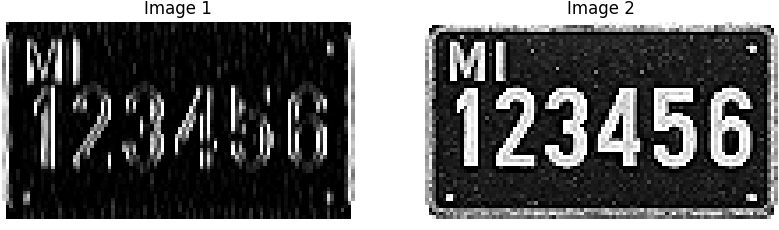
\includegraphics[width=0.85\linewidth]{W4Q3_edge_detection_plot.png}
\caption{Left: Vertical edge detection result. Right: sharpened image.}
\end{figure}
The first kernel, which is a vertical edge detection kernel, produces a filtered image in which vertical lines correspond to high pixel values and thus appear white; on the other hand, horizontal edges and uniform regions produce a low (or even negative) value, and are displayed as black. If we used the transpose of this kernel, we would detect horizontal edges instead.

The convolution with the second kernel sharpens the edges, making the contrast between the digits and the background of the car plate more apparent.

\end{document}